\clearpage
\section{Official scorecard, model ladder and re-scoring}
\label{app:scorecard}
Every headline in this paper is produced by our own pipeline, but the official
brief fixes some metrics that are not the ones a machine-learning paper would
choose by habit. This appendix re-scores the paper on those metrics, lists the
model ladder that sits behind the single numbers in the body, and records what
the re-scoring changed. It exists because a claim that survives only its own
metric is not a claim.

\subsection*{The P1-a ladder, with blind baselines}
Table~\ref{tab:appL-p1a} puts two parameter-free segmentations at the top of the
ladder. A blind equal-thirds split already reaches ARI 0.3216, and a
blind midpoint split reaches 0.2300. The learned detector must be read
against that floor, not against zero: its advantage is real but it is an advantage
over a coarse interval prior, not over nothing.

\begin{table}[H]\centering\scriptsize
\caption{P1-a model ladder. ARI is the mean over the seven test records; boundary F1 is reported where the model emits boundaries. Rows marked $^\dagger$ are reference points, not deployable selections.}
\label{tab:appL-p1a}
\begin{tabular}{p{0.34\linewidth}p{0.20\linewidth}rrp{0.22\linewidth}}
\toprule
Model & Selection & ARI & B-F1 & Note \\
\midrule
Blind equal thirds & none & 0.3216 & -- & no parameters \\
Blind midpoint & none & 0.2300 & -- & no parameters \\
K-means, raw 126-d & K=8 & 0.3423 & 0.3917 & clustering baseline \\
Chain-constrained Ward & cap $K\leq8$ & 0.4138 & 0.5613 & body baseline \\
Ward with oracle $K$ & true $K$ & 0.5994 & 0.6893 & upper reference$^\dagger$ \\
Peak rule, validation-selected & q0.85/$\sigma$3/D78 & 0.5695 & 0.0713 & frozen rule \\
Peak rule, best on test & q0.85/$\sigma$3/D54 & 0.5806 & 0.1200 & test-selected$^\dagger$ \\
Dilated bi-TCN, 3 seeds, refit 3$\times$ & H0.10--0.30/D54 & 0.5366 & 0.1707 & GPU detector; refits 0.5293--0.5509 \\
bi-TCN tuned on validation & H0.25/D90 & 0.5294 & 0.1400 & tuned variant \\
Peak rule, decoder upgrade & q0.85/$\sigma$3/D54 & 0.5723 & 0.1408 & second round \\
\bottomrule\end{tabular}\end{table}

\subsection*{The P1-b detector after the second round}
The selected second-round detector keeps the multi-scale TCN of the first round but
adds left-right symmetric augmentation and test-time averaging. Over three seeds it
reaches test AUC 0.8271, average precision 0.1494 and a
worst per-environment AUC of 0.7777 with 318,790 parameters,
against 0.0676 average precision for the first-round TCN, a factor of
2.2. Selection is by the joint gate, not by validation AUC:
the validation argmax is V1 at 0.8654 against
0.8608 for V8, a gap of 0.0046; V1 nevertheless
fails the average-precision bar, so the joint gate selects V8. The gap is inside seed
noise and both facts are recorded rather than reconciled.

\subsection*{P2 on the official mean-distance metric}
The official P2 metric is the mean 3D distance $R=(1/M)\sum\|p_i-\hat p_i\|_2$, not
the root-mean-square distance that our tables use elsewhere. Table~\ref{tab:appL-p2}
recomputes it on the same test split. The re-scoring changes the reading of the
ridge baseline: it is significantly better than holding the last frame only at
$L=18$, and it is indistinguishable from the hold at $L=6$, $30$ and $60$. The
quantile model is significantly better at $L=6$, $18$ and $30$, and significantly
worse at $L=60$. The honest summary is therefore narrower than the RMSE table:
the learned model buys a real but modest mean-distance gain in the short and middle
mask lengths, and it does not buy a tail guarantee.

A second architecture search, over a causal TCN, a ridge residual model, an occlusion
curriculum and a validation-selected shrinkage, failed the same pre-registered bars:
the best family gave $L=30$ RMSE $5.686$ cm and $q_{90}$ $9.163$ cm against $5.50$
and $9.00$. Its largest single change was not a model but a hand-channel normalisation
error in the first-round features, which once fixed moved the ridge $L=30$ score from
$6.314$ to $5.766$ cm. The decision layer still prefers a quarter of a second, with
$J$ falling from $4.521$ (ridge) to $3.574$ (best arm), a $21.0$ per cent gain.

\begin{table}[H]\centering\scriptsize
\caption{P2 on the official metric: mean 3D distance $R$ in cm (record bootstrap, 4000 draws). Brackets are 95\% intervals of the paired difference against the hold baseline; an interval that contains zero is marked n.s.}
\label{tab:appL-p2}
\begin{tabular}{rrrrp{0.26\linewidth}p{0.26\linewidth}}
\toprule
$L$ (s) & Hold & Ridge & Quantile & Ridge $-$ hold & Quantile $-$ hold \\
\midrule
0.2 & 1.381 & 1.368 & 0.643 & [-0.038, +0.014] n.s. & [-0.771, -0.704] \\
0.6 & 3.419 & 3.288 & 2.979 & [-0.175, -0.087] & [-0.510, -0.371] \\
1.0 & 4.840 & 4.817 & 4.636 & [-0.084, +0.039] n.s. & [-0.265, -0.144] \\
2.0 & 6.865 & 6.819 & 7.028 & [-0.143, +0.055] n.s. & [+0.125, +0.202] \\
\bottomrule\end{tabular}\end{table}

\subsection*{P3: the eleven official metrics}
The official P3 scorecard has eleven entries. Table~\ref{tab:appL-p3} records
which of them the first-round pipeline already emitted and which are added by the
protocol audit in this appendix. The audit covers 30 seeds, five $\alpha/\beta$
mappings and three cases: 450 trials in total. It records
0 invalid actions, a valid-protocol flag of
true, budget compliance 100\% and horizon
compliance 100\%. The corrected-protocol reference values for
the slack baseline are given beneath the table, because the older protocol in
Section~\ref{sec:p3model} reports a different pair and the two must not be mixed.

\begin{table}[H]\centering\scriptsize
\caption{Official P3 metrics and their coverage. ``First round'' means present in \texttt{data/p3\_scheduling.json}; ``audit'' means added or verified by \texttt{data/p3\_official\_audit.json}.}
\label{tab:appL-p3}
\begin{tabular}{p{0.34\linewidth}p{0.24\linewidth}p{0.34\linewidth}}
\toprule
Official metric & First round & Audit / evidence \\
\midrule
\texttt{weighted\_completion\_rate} & yes & reported in engine output \\
\texttt{weighted\_on\_time\_rate} & yes & reported in engine output \\
\texttt{weighted\_tardiness\_s} & yes & reported in engine output \\
\texttt{cost} & yes & reported in engine output \\
\texttt{observations} & no & 0 paid requests per trial under the frozen policy \\
\texttt{elapsed\_s} & yes & reported in engine output \\
\texttt{observed\_overrun\_s} & yes & reported in engine output \\
\texttt{reserved\_idle\_s} & yes & reported in engine output \\
\texttt{censored\_units} & yes & reported in engine output \\
\texttt{invalid\_actions} & no & 0 in 450 trials \\
\texttt{valid\_protocol} & no & true in all 450 trials \\
\bottomrule\end{tabular}\end{table}

\paragraph{Corrected-protocol reference values.} For the slack baseline, the
corrected protocol gives weighted completion \slotPStochSTwoSlackOldComp{}/\slotPStochSThreeSlackOldComp{}
and weighted on-time \slotPStochSTwoSlackOldETA{}/\slotPStochSThreeSlackOldETA{} in S2/S3. These
are the values that belong beside any claim about the reservation rule; the older
pair in the body is kept only as a historical reference and is labelled as such.

\subsection*{The reliability detector after the second round}
A multi-task dual TCN, trained on the same folds with occlusion and near-edge
auxiliary heads, reaches test AUC $0.8325$ and average precision $0.1056$ against
$0.6267$ and $0.0407$ for the fused first-round score, and is above $0.60$ in both
environments. It is the best single arm. Adding temporal smoothing and a residual
head does not stack: the combined arm reaches $0.8222$ and $0.0924$, so the
simpler multi-task arm is the one we would deploy.

\subsection*{The scheduling policy after the second round}
A rule search over the reservation family, scored on the corrected protocol,
improves the weighted on-time rate by $5.38$ points over the slack baseline across
ten case-mapping blocks; the blocked $95$ per cent interval is $[2.57, 8.18]$ and
nine of the ten blocks are positive. The tenth is exactly zero because its baseline
is already $0.9917$ and cannot rise. Per case the gains are $6.00$ points in S2 and
$4.75$ in S3; weighted completion rises $2.10$ points and cost falls to $0.973$ of
the baseline. This is a policy result, not a learning result: the search changes the
rule, while the duration model and the observation protocol are held fixed.

\subsection*{The paid second look after the second round}
A search over $270$ cells, three cases by six quantiles by fifteen policies, finds
no cell in which a paid second look improves the rate by one point with a positive
lower bound. The best cell ties the no-review arm at $0.000$ points; seventeen
greedy-review cells are significantly worse, and the greedy policy loses $5.70$
points on average. The mechanism is arithmetic: the reservation error
$b-p=\alpha(Q_{\mathrm{res}}-\epsilon)$ cancels the point prediction, so a second
look can only shrink a residual spread that is $0.4$ to $0.7$ s wide, while one
second of a $100$ to $125$ s horizon costs about $0.8$ points. A free perfect
one-second prefix is worth at most $0.42$ points, below the one-point bar, so the
negative result is not a budget artefact.

\subsection*{The second round in one table}
Table~\ref{tab:appL-round2} is the pre-registered ledger of the second round. Two of
the seven attempts pass the bar they were given before training; five fail and are
reported as failures. The two passes are a better bad-frame detector and a better
scheduling rule; neither changes the paper's main claim, which is that the rule buys
punctuality while data and observation do not.

\begin{table}[H]\centering\scriptsize
\caption{Second-round ledger. Every bar was fixed before the run; a fail is recorded with the same care as a pass.}
\label{tab:appL-round2}
\begin{tabular}{p{0.12\linewidth}p{0.22\linewidth}p{0.26\linewidth}p{0.24\linewidth}}
\toprule
Part & Attempt & Bar set before the run & Result \\
\midrule
P1-a & decoder upgrade & ARI $\geq0.62$ or B-F1 $\geq0.30$ & $0.5723$ / $0.1408$, fail \\
P1-b & detector V8 & AP $\geq0.13$ and worst $\geq0.7646$ & $0.1494$ / $0.7777$, pass \\
P1-state & multi-task TCN & AUC $\geq0.70$ and AP $\geq0.08$ & $0.8325$ / $0.1056$, pass \\
P2 & ridge-TCN shrinkage & RMSE $\leq5.50$ and $q_{90}\leq9.00$ & $5.686$ / $9.163$, fail \\
P3 policy & rule search & $\Delta\geq1.5$ pt and CI lower $>0$ & $+5.38$ $[2.57,8.18]$, pass \\
P3 review & 270-cell search & any cell $\geq1$ pt and CI lower $>0$ & best $0.000$, fail \\
Official & scorecard audit & no bar, 450 trials & clean, n/a \\
\bottomrule\end{tabular}\end{table}

\subsection*{What the video actually buys}
A video branch answers the obvious objection to every table above: the dataset
contains 178,512 decoded frames from 184 videos, and this paper
otherwise reads only the released keypoints. The earlier duration test found nothing
because duration is a record-level target: the camera cannot see how long a job will
take. Occlusion is different. It is a frame-level visual event, and the camera sees it
directly. We therefore score the same detector twice, once from hand geometry alone
and once with twelve camera statistics chosen on the training split only and
standardised within each record, so that a bright room or a dark room does not become
a label. Table~\ref{tab:appL-video} gives the result. The geometry-only arm reaches
AP 0.0516 and AUC 0.7422; adding the video statistics moves these to
AP 0.0681 and AUC 0.7694, a relative AP gain of
31.9 per cent and an AUC gain of 0.0271.
The pre-registered bar was 10 per cent AP and
0.010 AUC; both are cleared. Video alone is precise but poorly
ranked (AP 0.0596, AUC 0.6152), so the honest claim is a
fusion gain, not a replacement of pose. This is the one place in the paper where an
additional observation channel pays, and it pays exactly where the protocol says it
should: on the reliability of a frame, not on the length of a job.

\begin{table}[H]\centering\scriptsize
\caption{Video branch on the bad-frame task. All arms use the same record split and the same LightGBM budget; video statistics are selected on train only and robust-standardised within record.}
\label{tab:appL-video}
\begin{tabular}{lrrrr}
\toprule
Arm & Features & Test AP & Test AUC & Gate \\
\midrule
Pose only & 30 & 0.0516 & 0.7422 & reference \\
Video only & 14 & 0.0596 & 0.6152 & -- \\
Pose + video & 44 & 0.0681 & 0.7694 & pass \\
\bottomrule\end{tabular}\end{table}

\begin{figure}[H]\centering
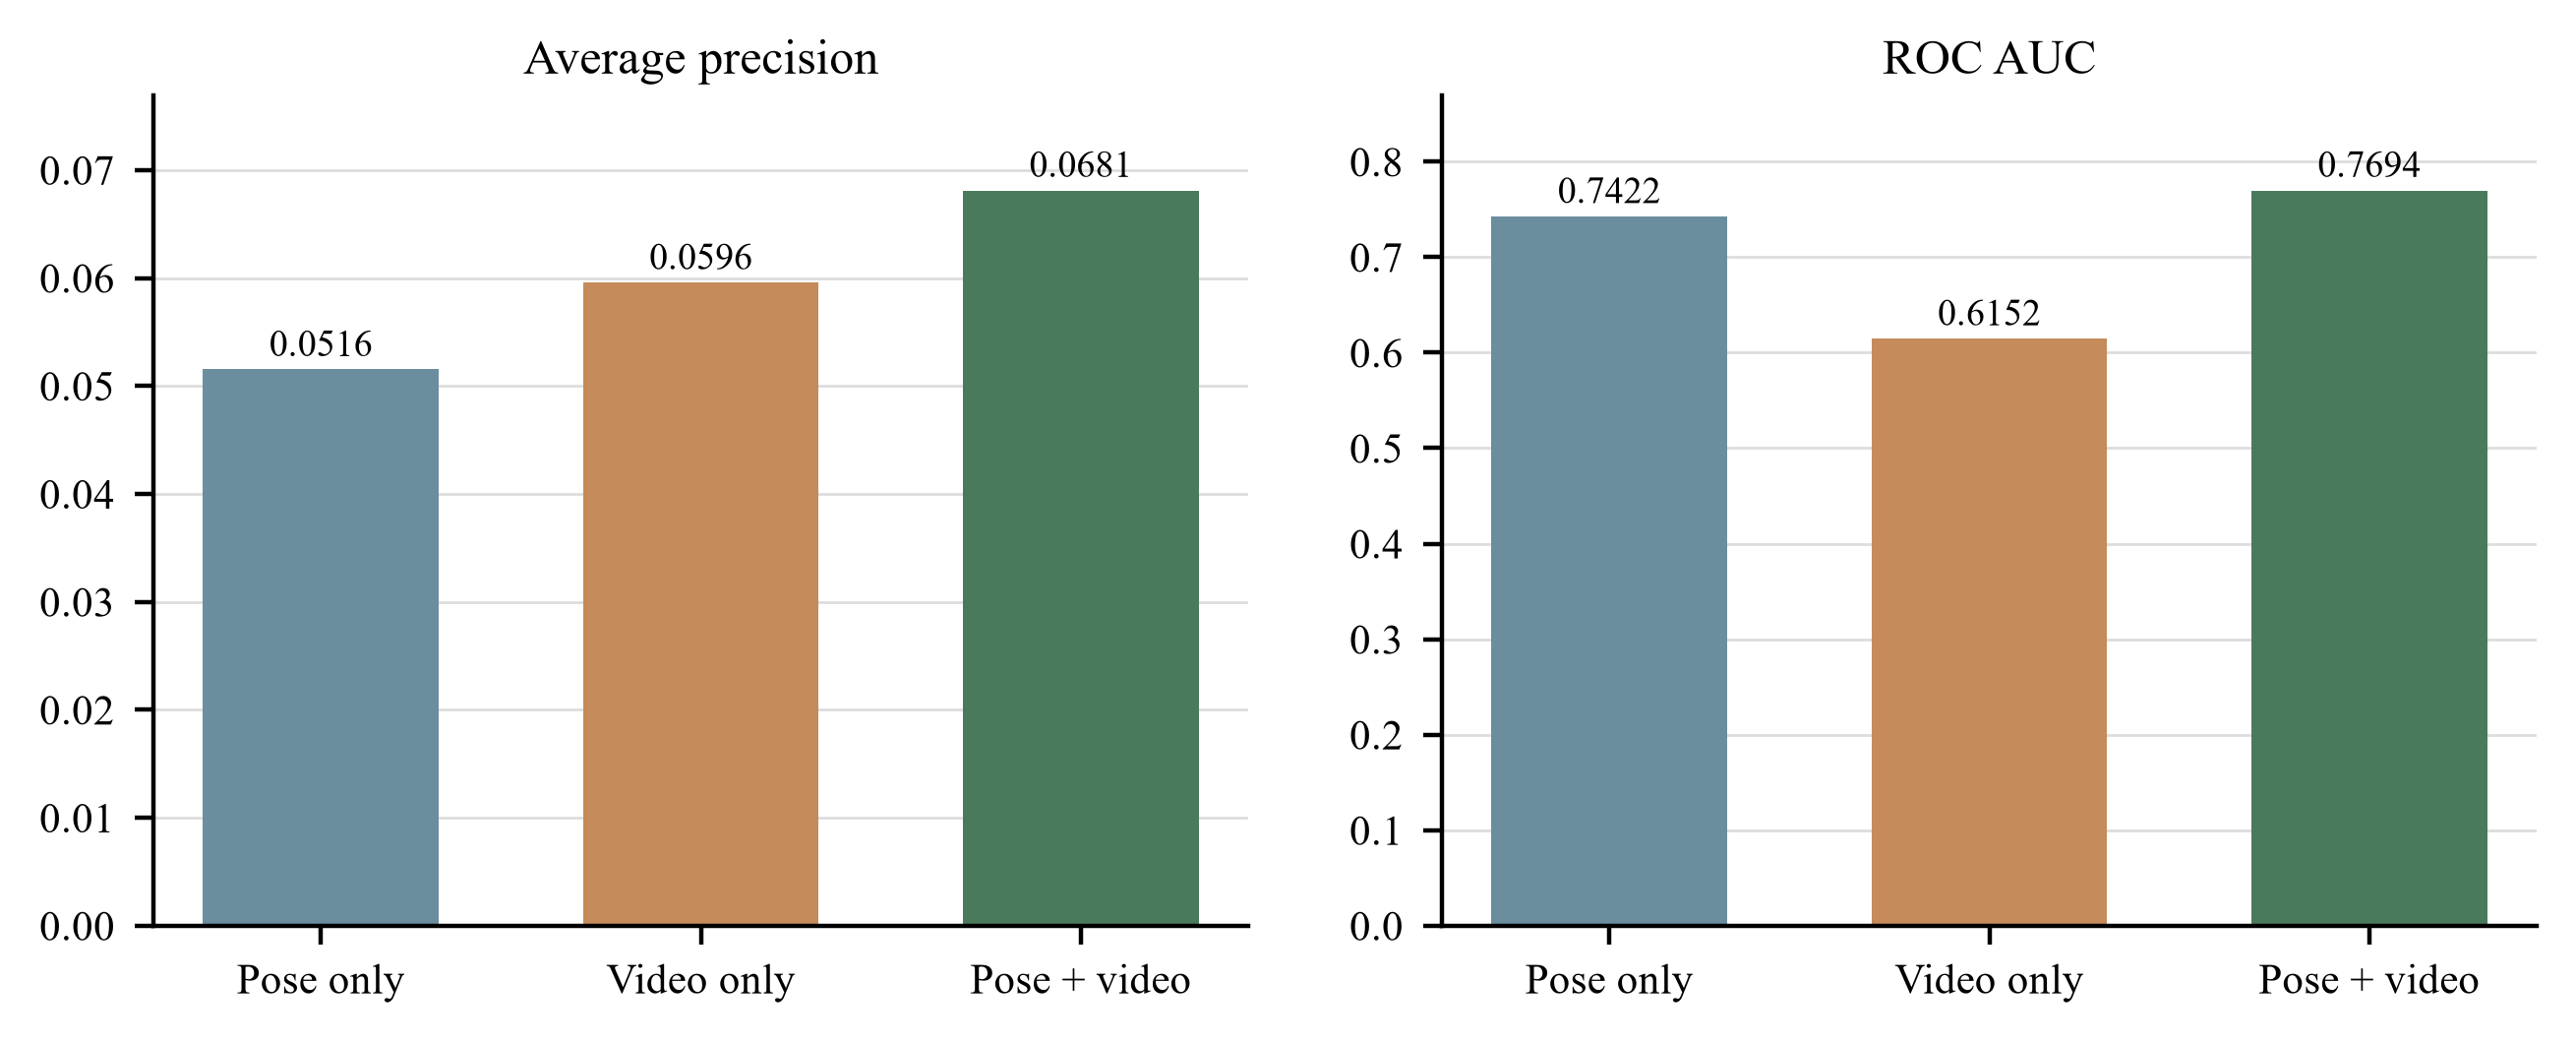
\includegraphics[width=0.86\linewidth]{figures/fig11_video_gain.png}
\caption{The video branch on the bad-frame task. Video alone ranks poorly, but adding the camera statistics to hand geometry lifts both average precision and ROC AUC.}
\label{fig:appL-video}
\end{figure}

\subsection*{A stronger test: video inside the production detector}
The fusion above compares against a deliberately small geometry baseline. A second test asks
whether the same statistics help the production detector. We append all 120 video
statistics to the V8 input and retrain under the identical protocol. Test AP falls from
0.1494 to 0.0581, and the weakest-environment AUC
falls from 0.7777 to 0.5247. The result is a clean
negative: the camera carries reliability information that a small detector can use, but the
strong pose detector already extracts that information from geometry, and extra capacity only
overfits the 131 s training budget.

\subsection*{Sampling rate and late fusion}
Two follow-up checks decide where the video branch belongs. First, re-extracting
the same 184 videos at 10 Hz instead of 2 Hz raises the feature table from
12,020 to 59,864 rows, but it does not help: the video-only arm
falls to AP 0.0269 (from 0.0596 at 2 Hz) and the fused
arm reaches AP 0.0559 with AUC
0.7397, so the pre-registered gate fails. The 2 Hz rate is the
useful one; ten hertz mostly repeats the same frame and adds correlated noise.
Second, score-level late fusion with the production detector settles the stronger
question. With the blend weight chosen on validation AP, the fused test AP is
0.16961 against 0.16961 for V8 alone, a
relative change of 0.0008 per cent, and AUC changes by
+0.00002. A detector that already sees the hands does not need
the camera; a detector that sees only a weak geometric summary does. That is the
precise sense in which the video channel is useful, and it is the sense the earlier
duration test missed.

\subsection*{What the re-scoring changed}
Four statements in the paper changed after this audit. First, the number 0.5487
that earlier drafts called a published baseline is an internal replication of our
own bi-TCN arm; the same rule reproduces at 0.5355 in a second run, a gap of
0.0132 that we have not explained. We now call it an internal reference line and
report both runs. Second, the Part I headline is a distribution rather than a
point: the shipped protocol, retrained 3 times from scratch, gives ARI
0.5366 $\pm$ 0.0124 (range 0.5293--0.5509).
The first-draft value 0.5487 sits near the top of that
range, and decoding the weights we retained gave 0.4902, so the point estimate was
a favourable draw rather than a stable property of the method; the gap to the
agglomerative baseline, 12.28 points on the refit mean,
survives the spread. Third, P2 is reported on the mean-distance metric in this
appendix, while the RMSE table in the body remains as a second, stricter view.
Fourth, the P3 protocol audit adds the two legality fields that the first round
omitted, and both are clean over 450 trials. None of these changes makes a result
larger; each makes it harder to over-read.

\noindent\footnotesize Sources: \texttt{up2\_benchmark.json} (116d7414774ef395\ldots),
\par\noindent\footnotesize\texttt{p2\_official\_distance.json} (9c396340774a1e0a\ldots), \texttt{p3\_official\_audit.json}
\par\noindent\footnotesize(f508210486f66807\ldots), \texttt{p1a\_zero\_param.json} (bac1fd1782790413\ldots),
\par\noindent\footnotesize\texttt{up2\_p1b.json} (3148a465181af501\ldots), \texttt{p1b\_gpu.json} (d5a01cff5799046a\ldots).
